\section{Overview}
\label{sec:inference:overview}

% Figure \ref{fig:overview_app} shows a high-level overview of the entire application with the following main parts:
% Figure \ref{fig:overview_app} shows a high-level overview of the entire application with these four main parts:
Figure \ref{fig:overview_app} shows a high-level overview of the entire application consisting of these four parts:
% The four main parts are the following:
\begin{enumerate}
  \item Camera Library (\texttt{libcamera.so})
  \item Python Package (\texttt{fhnwtoys})
  \item User Interface Class (\texttt{ui.py})
  \item Inference Application (\texttt{aionfpga.py})
\end{enumerate}

% explain the four parts that the app uses:
% Camera Library
% Package
% User Interface Class
% inference application itself

% The camera library is a shared library which initializes and  the camera
% The interface between the application and the camera is realized in a shared library.
% The camera interface is realized in a shared library written in C++.
% The camera interface is written in C++ and compiled to a shared library.
The camera interface is written in C++ and compiled into a shared library (\texttt{.so}).
% This allows the inference application to load the camera library and access its memory.
% This allows the inference application to load the camera library and share its memory space.
% This allows the inference application to load the camera library and share their memory space.
% This allows the inference application to load the camera library and share their memory space.
This allows the inference application to load the camera library into its memory space (see section \ref{sec:inference:camera_library}).

The \texttt{fhnwtoys} Python package provides access to various settings and constants.

The \acrlong{ui} class serves as an interface between the inference application and the display.
% It features two methods which make it easy to update the user interface screens.
It features two methods to easily update the user interface screens.

% The inference application itself uses the other three components to control the
The inference application itself uses the other three components to acquire frames, run inference and display the classification results on the screen.

\begin{figure}
  \centering
  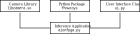
\includegraphics[width=\textwidth]{overview_app}
  \caption{High-level overview of the entire application}
  \label{fig:overview_app}
\end{figure}
